\documentclass[letterpaper, 8pt]{extarticle}
\usepackage{amssymb,amsmath,amsthm,amsfonts}
\usepackage{multicol,multirow}
\usepackage{calc}
\usepackage{ifthen}
\usepackage[landscape]{geometry}
\usepackage[colorlinks=true,citecolor=blue,linkcolor=blue]{hyperref}
\usepackage{booktabs}
\usepackage{ulem}
\usepackage{enumitem}
\usepackage{tabulary}
\usepackage{graphicx}
\usepackage{siunitx}
\usepackage{tikz}
\usepackage{derivative}
\usepackage{svg}
\usepackage{listings}


\ifthenelse{\lengthtest { \paperwidth = 11in}}
    { \geometry{top=.35in,left=.1in,right=.1in,bottom=.35in} }
	{\ifthenelse{ \lengthtest{ \paperwidth = 297mm}}
		{\geometry{top=1cm,left=1cm,right=1cm,bottom=1cm} }
		{\geometry{top=1cm,left=1cm,right=1cm,bottom=1cm} }
	}

\newenvironment{Figure}
  {\par\medskip\noindent\minipage}
  {\endminipage\par\medskip}

\pagestyle{empty}
\makeatletter
\renewcommand{\section}{\@startsection{section}{1}{0mm}%
                                {-1ex plus -.5ex minus -.2ex}%
                                {0.5ex plus .2ex}%x
                                {\normalfont\normalsize\bfseries}}
\renewcommand{\subsection}{\@startsection{subsection}{2}{0mm}%
                                {-1explus -.5ex minus -.2ex}%
                                {0.5ex plus .2ex}%
                                {\normalfont\small\bfseries}}
\renewcommand{\subsubsection}{\@startsection{subsubsection}{3}{0mm}%
                                {-1ex plus -.5ex minus -.2ex}%
                                {1ex plus .2ex}%
                                {\normalfont\tiny\bfseries}}
\makeatother
\setcounter{secnumdepth}{0}
\setlength{\parindent}{0pt}
\setlength{\parskip}{0pt plus 0.5ex}
% -----------------------------------------------------------------------
% \tymin=37pt
% \tymax=\maxdimen

% Custom siunitx defs
\DeclareSIUnit\noop{\relax}

\NewDocumentCommand\prefixvalue{m}{%
\qty[prefix-mode=extract-exponent,print-unity-mantissa=false]{1}{#1\noop}
}

% Shorthand definitions
\newcommand{\To}{\Rightarrow}

% condense itemize & enumerate
\let\olditemize=\itemize \let\endolditemize=\enditemize \renewenvironment{itemize}{\olditemize \itemsep0em}{\endolditemize}
\let\oldenumerate=\enumerate \let\endoldenumerate=\endenumerate \renewenvironment{enumerate}{\oldenumerate \itemsep0em}{\endoldenumerate}
\setlist[itemize]{align=parleft,left=0pt..1em}
\setlist[enumerate]{align=parleft,left=0pt..1em}

\title{2LC3}

\begin{document}

\raggedright
\tiny

\begin{center}
  {\textbf{2ME3 - OSCS}} \\
\end{center}
\begin{multicols*}{6}
  \setlength{\premulticols}{1pt}
  \setlength{\postmulticols}{1pt}
  \setlength{\multicolsep}{1pt}
  \setlength{\columnsep}{2pt}

  \section{Programming Paradigms}
  \textbf{Procedural:} C, Assembly
  \textbf{Object-Oriented:} C\#, C++, Python, Java, Scala
  \textbf{Functional:} Haskell, Elm, Scala
  \textbf{Logical:} Prolog

  \section{CS vs SE}
  \textbf{CS:} More theory focused, Algorithms

  \textbf{SE:} Practical / Implementation, Design,
  Regulated by CEAB, not taken too seriously by PEO

  \textbf{PEO:} Professional Engineers of Ontario, Licensing and accreditation for Engineering \\
  4 years of practical experience (3 with an accredited degree), law / ethics exam, yearly fees \\
  Regulation, enforcement, discipline \\
  Has legal authority to fine companies misusing the term engineer \\
  Iron Ring just means you graduated, pretty useless, get it at the Kipling ceremony

  \textbf{CEAB:} Canadian Engineering Accreditation Board,
  determines if an engineering program gets approved.

  \section{SDLC}
  \begin{itemize}
    \item Requirement Analysis
          \begin{itemize}
            \item Getting input from stakeholders (customers, salespeople, industry experts, programmers.)
            \item What the software does
            \item Software Requirements Specification (SRS)
                  \begin{itemize}
                    \item Document describing what the software is, what it does, etc.
                  \end{itemize}
            \item Functional Requirements
                  \begin{itemize}
                    \item What the software actually does
                    \item Must be:
                          \begin{itemize}
                            \item Atomic: Each requirement should cover exactly one function of the software
                            \item Precise: Requirements should not be ambiguous
                            \item Verifiable: Must be testable to determine whether the requirement is actually met
                          \end{itemize}
                    \item Things you can \textbf{prove} using logic / discrete math
                    \item ``The software shall...''
                  \end{itemize}
            \item Non-functional Requirements
                  \begin{itemize}
                    \item Usability, performance, security
                  \end{itemize}
          \end{itemize}
    \item Specification and Design
          \begin{itemize}
            \item Determining how the software will meet requirements specified in SRS document.
            \item Modules, classes \& objects, packages
            \item Libraries \& APIs
            \item Class Diagrams
            \item What the code does, what should functions output given specific inputs
          \end{itemize}
    \item Coding
          \begin{itemize}
            \item How specification is implemented
          \end{itemize}
    \item Deployment and Maintenance
  \end{itemize}
  \subsection{Contract between client and developers}
  \textbf{Scope:} Important for clients, allows for specifying what should be included.
  \textbf{Out of scope:} Important for devs,
  allows specifying what the program will not be responsible for,
  preventing feature creep.

  \subsection{Methodologies}
  \textbf{Waterfall:} Finish one phase completely, then start the next.
  Each phase has mini-plan, and waterfalls into next.
  Drawback is that missing details in one phase
  end up causing issues in future phases.
  \includegraphics[width=0.8\linewidth]{waterfall.png}

  \textbf{Agile:} Separate product into cycles
  and deliver working product quickly.
  Essentially small loops of waterfall,
  each only concerned about a small part of each step
  (eg requirements can be loose at the beginning, sprints may not produce working code).
  Constant feedback allows for issues to be spotted before they become massive problems.
  Lots of customer interaction can lead the project astray.
  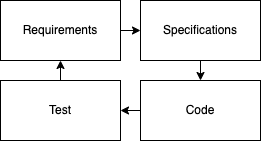
\includegraphics[width=0.8\linewidth]{agile.png}

  \textbf{Spiral:} Similar to agile, but a prototype is made each sprint cycle.

  \section{Good Software}
  Efficient, timely, performant.
  \textbf{Maintainable:} Salable, Extendable, Reusable, Readable
  High Usability.
  \textbf{Reliable:} The ability of a system or component to perform
  required functions under static conditions for a specific period
  \textbf{Correctness:} Meets (specified) requirements.
  Correctness is achieved if it behaves exactly as intended
  for all of its use-cases. (eg passes tests)
  \textbf{Robust:} Meets unspecified requirements.
  The ability of a system to cope with errors during execution,
  and cope with erroneous input (eg the program should fail gracefully)
  \textbf{Distribution of cost in development}
  40\% of cost on initial development. 60\% on maintenance.
  Of that, 20\% is on making sure things are correct,
  20\% is adaptive (correcting things the client wants to be fixed),
  20\% is improvement.

  \section{Object-Oriented Programming}
  \subsection{Encapsulation}
  Safeguarding the content of a class from direct outside access.
  Make certain fields private, access them through public getters and setters.
  Separation of concerns.
  \textbf{Modularity:} Programs should be made up of independent, interchangeable parts
  Information Hiding
  Single responsibility Principle
  \textbf{Open-close principle:} objects should be open for extension,
  but closed for modification.

  \subsection{Relationships between Classes}
  \subsubsection{Inheritance}
  Is-a relationship. Good for reusability, code does not need to be rewritten.
  \subsubsection{Aggregation}
  Has-a relationship: A has-a B, then A has an instance of B.
  Must be mandatory upon creation, otherwise it is simply association / dependence
  \subsubsection{Composition}
  Part-of relationship: A part-of B, A can't exist without B, and vice-versa.
  A subset of aggregation.
  \subsubsection{Dependence / Association}
  Uses-a relationship: A uses-a B, then A creates an object of B inside a method.
  Association is generally between unrelated classes. % check this, not too certain

  \subsection{Abstraction}
  Hides complexity from users, showing only relevant info.
  Implementation hidden using abstract (partially abstract) classes,
  or interfaces (fully abstract).

  \subsection{Polymorphism}
  Performing a certain action in different ways (eg animals can make different noises).
  \textbf{Method overloading:} various methods with the same name but different parameters.
  \textbf{Method overriding:} child class overrides a method of its parent.

  \section{UML Diagrams}
  \begin{center}
    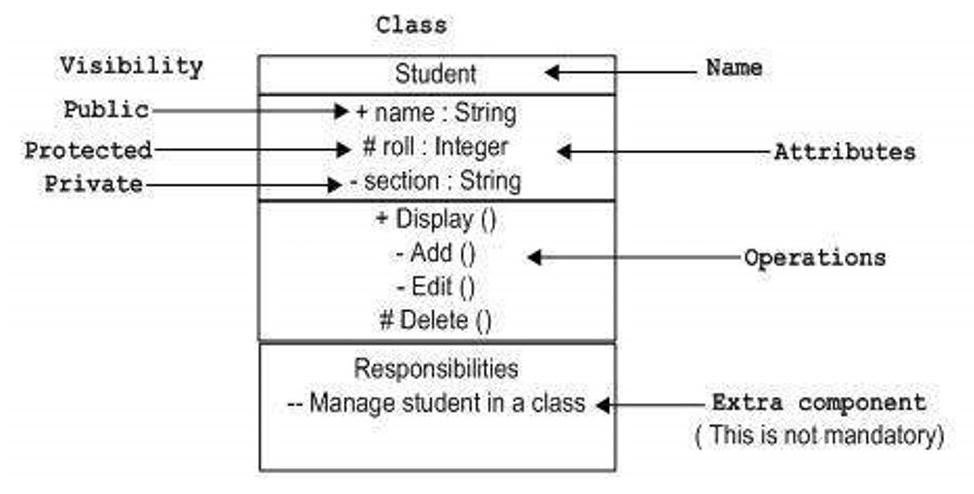
\includegraphics[width=.9\linewidth]{uml-class.png}
    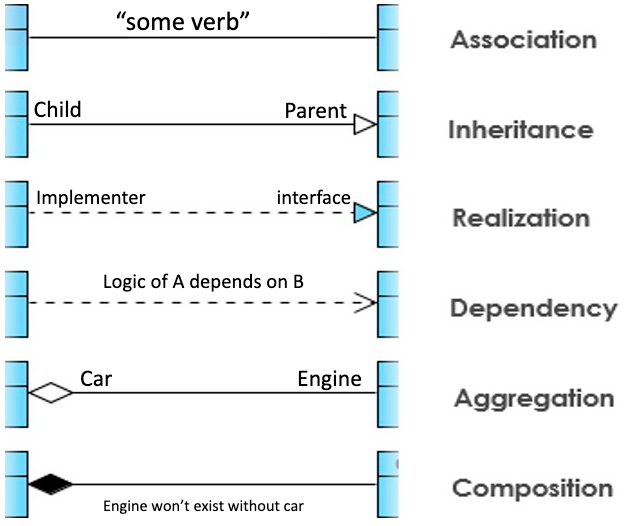
\includegraphics[width=.9\linewidth]{uml-arrows.png}
  \end{center}

  \section{Java}
  \subsection{Abstract Class}
  Can have abstract and non-abstract method.
  Can have non-final variables
  Can have final, non-final, static, and non-static variables.
  Can provide implementation of abstract class.
  Uses ``extends''
  Can only extend one other class, but can implement multiple interfaces.
  Does not support multiple inheritance.
  Can have private members.
  \subsection{Interface}
  Can only have abstract methods.
  Variables are final by default.
  Can only have static and final variables.
  Can't provide implementation of abstract class.
  Can extend one or more Java interfaces.
  Supports multiple inheritance.
  Members are public by default.

  \section{Multiple Inheritance}
  When a class inherits from more than one class.
  Constructors are called in the order they are inherited.

  \section{SOLID}
  \textbf{Single responsibility principle:}
  Each class should have one and only one responsibility.

  \textbf{Open/Closed Principle:}
  Classes should be open for extension but closed for modification

  \textbf{Liskov's Substitution Principle:}
  Parent classes should be easily substituted with child classes without
  the application malfunctioning.
  \textbf{Interface Segregation Principle:}
  Many client-specific interfaces are better than one general interface.
  \textbf{Dependency Inversion Principle:}
  Classes should depend on abstraction, but not on concretion.
  Aka, have an interface which allows for communication with concrete classes.
  If class A changes, class B should not be affected.

  \section{Design Principles}
  \subsection{Information Hiding}
  AKA Single Responsibility Principle
  AKA Encapsulation

  Changes to a class should have \textbf{minimal} impact on other code:
  The API for a class should be completely independent of the implementation.


  \subsection{Open-Closed}
  Entities should be open for extension, but closed for modification.

  In other words, the original functionality should remain static,
  while allowing new functionality to be added on,
  without the original source needing to be modified.

  \subsection{Design for Interfaces}
  AKA Dependency Inversion
  Don't depend on concrete classes, use interfaces instead.

  \section{Creational Patterns}
  \subsection{Factory}
  Provides an interface for creating objects in a superclass,
  allows subclasses to alter type of objects that will be created.

  \begin{enumerate}
    \item Have an interface A
          \begin{lstlisting}[language=Java, breaklines=true]
public interface Factory {
  public Enemy spawn();
}
        \end{lstlisting}
    \item Have factory ``products'' implement A
          \begin{lstlisting}[language=Java, breaklines=true]
public abstract class Enemy {
  protected int health;
  protected int strength;
  public abstract void takeDamage(int damage);
  public abstract void attack();
}
        \end{lstlisting}
    \item Have the factory function return an object of type A
          \begin{lstlisting}[language=Java, breaklines=true]
public class AverageSpawner implements Factory{
  @Override
  public Enemy spawn() {
    Random r = new Random();
    double k;
    k = r.nextDouble();
    if(k < 0.65) {
      return new Minion();
    }
    else if(k < 0.9) {
      return new Elite();
    }
    else {
      return new Boss();
    }
  }
}
        \end{lstlisting}
    \item Let clients get ``products'' through the factory function
  \end{enumerate}

  \begin{center}
    \includegraphics[width=0.9\linewidth]{factory.png}
    \includegraphics[width=0.9\linewidth]{factory-example.png}
  \end{center}

  \textbf{Advantages:}
  Can switch out factories at runtime to change what's being produced.
  Object instantiation is encapsulated.
  Single Responsibility Principle - can move product creation into a separate area,
  making code easier to support.
  Open Closed Principle - can introduce new types of products without
  affecting existing code.

  \textbf{Disadvantages:}
  Code can become complex due to subclasses.

  \subsection{Singleton}
  % TODO: add singleton

  \section{Structural Patterns}
  \subsection{Decorator}
  Lets you attach new behaviors to objects by putting them in special wrappers
  that contain the behaviors.

  \begin{enumerate}
    \item Create interface A
          \begin{lstlisting}[language=Java, breaklines=true]
public interface Burrito {
  public double getCost();
  public String getString();
}
        \end{lstlisting}
    \item Create base class B that implements A
          \begin{lstlisting}[language=Java, breaklines=true]
public class ChickenBurrito implements Burrito{
  public ChickenBurrito() {}
  public String getString() {
	return "Chicken" + "$12.00";
  }
  public double getCost() {
    return 12.00;
  }
}
        \end{lstlisting}
    \item Create decorator class C that implements A,
          that holds an instance of B,
          which is received through constructor
          \begin{lstlisting}[language=Java, breaklines=true]
public abstract class BurritoDecorator implements Burrito {
  protected Burrito burrito;
  public BurritoDecorator
      (Burrito burrito) {
    this.burrito = burrito;
  }
  @Override
  public abstract double getCost();
  @Override
  public abstract String getString();
}
        \end{lstlisting}
    \item Create decorators by extending C and using super
          \begin{lstlisting}[language=Java, breaklines=true]
public class Guac extends BurritoDecorator {
  public Guac(Burrito burrito) {
	super(burrito);
  }
  @Override
  public double getCost() {
	return 1.50
    + burrito.getCost();
  }
  @Override
  public String getString() {
	return burrito.getString() 
    + "\n--Guac + "$1.50";
  }
}\end{lstlisting}
  \end{enumerate}

  \begin{center}
    \includegraphics[width=0.8\linewidth]{decorator.png}
    \includegraphics[width=0.8\linewidth]{decorator-example.png}
  \end{center}

  Decorators are both the original component, and also use the original component.

  \textbf{Advantages:}
  Extensibility of code, new decor can just extend decorator interface.
  Greater flexibility, able to add or remove decorators at runtime.
  Simplifies coding, don't have to put all the functionality into the object.
  Single Responsibility Principle, larger classes can be broken down into several smaller ones.

  \textbf{Disadvantages:}
  Code can be harder to maintain, decreases as number of decorator classes grows.
  Hard to remove wrappers.
  Hard to implement decorators in a way that doesn't depend on ordering.

  \subsection{Adapter}
  % TODO: add adapter

  \subsection{Proxy}
  % TODO: add proxy

  \section{Behavioral Patterns}
  \subsection{Strategy}
  Define a family of algorithms, put them each in separate classes,
  and make their objects interchangeable.
  \begin{enumerate}
    \item Create a strategy interface
          \begin{lstlisting}[language=Java, breaklines=true]
public interface Sorter {
  public void 
    sort(ArrayList<Double> data);
}
        \end{lstlisting}
    \item Create concrete strategies that implement the interface
          \begin{lstlisting}[language=Java, breaklines=true]
public class DefaultSorter implements Sorter{
  @Override
  public void 
    sort(ArrayList<Double> data) {
    System.out
        .println("Default Sort");
    Collections.sort(data);
  }
}
        \end{lstlisting}
    \item Create a context to store the strategy
          \begin{lstlisting}[language=Java, breaklines=true]
public class SensorData {
  private ArrayList<Double> data = new ArrayList<Double>();
  private Sorter sort;
  public SensorData() {
  	sort = new DefaultSorter();
  }
  public void 
    addValue(double value) {
  	data.add(value);
  }
  public void setSort(Sorter sort) {
  	this.sort = sort;
  }
  public void print() {
  	System.out
      .println(data.toString());
  }
  public void sort() {
  	sort.sort(data);
  }
}

        \end{lstlisting}
  \end{enumerate}
  \begin{center}
    \includegraphics[height=4cm]{strategy.png}
    \includegraphics[width=0.8\linewidth]{strategy-example.png}
  \end{center}

  \textbf{Advantages:}
  Open-Closed Principle - Introducing new strategies without changing the encapsulation code,
  hiding of algorithm from application.
  Algorithms used by object can be changed at runtime.
  More maintainable, usable, extensible.

  \textbf{Disadvantages:}
  Overly complex if there are only a few algorithms needed.
  Must be aware of the difference between algorithms to pick the right one.

  \subsection{Observer}
  % TODO: add java code
  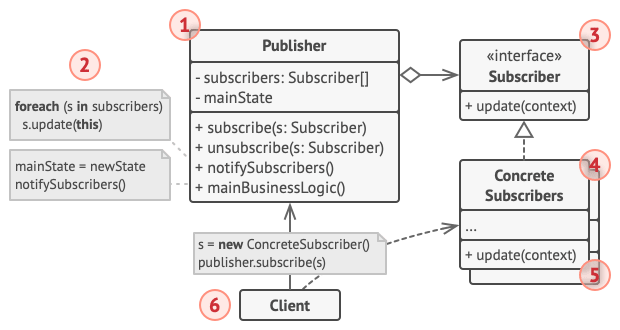
\includegraphics[width=\linewidth]{observer-example.png}
  Publisher calls update() on subscribers when needed. Subscribers can be added or removed at runtime.
  \textbf{Advantages:} Open-Closed Principle, can add new subscribers without changing the publisher.
  Can establish Relationships between objects at runtime.

  \textbf{Disadvantages:} Subscribers are notified in random order.

  \subsection{Command}
  \tikz[remember picture,overlay] \node[opacity=0.2,inner sep=0pt] at (current page.center){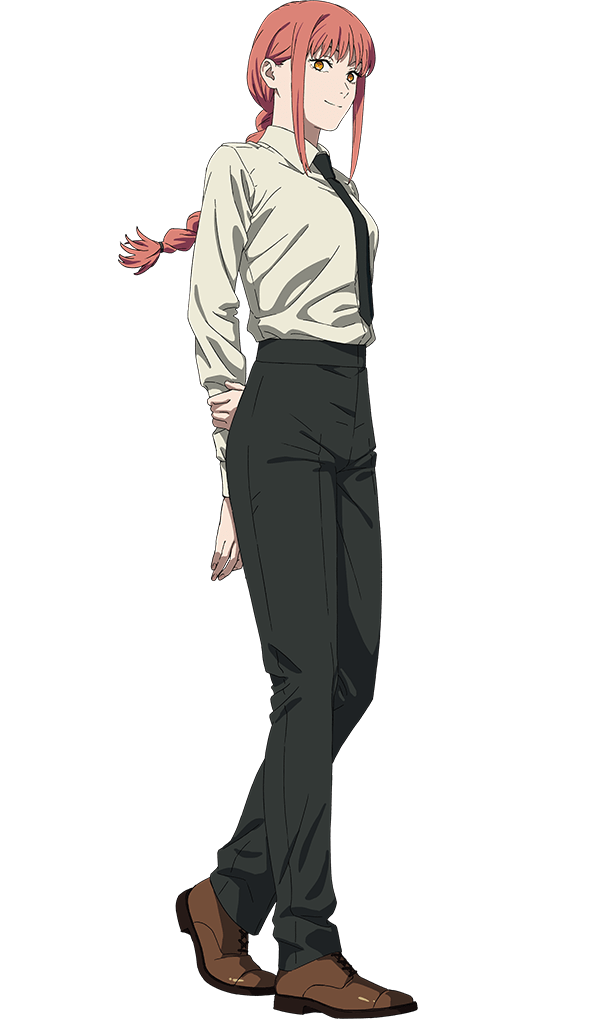
\includegraphics[height=0.8\paperheight]{Makima_anime_design_2.png}};
  % TODO: add command

  \section{Formal Specification}
  Form: $(\forall x : \mathbb{N} \mid R : P)$,
  where $\forall$ is a quantifier, $x$ is a variable, $\mathbb{N}$ is the type of variable,
  $R$ is the range over which the predicate is to be executed, and $P$ is the predicate.

  \section{Testing}
  \textbf{Unit Testing:} Test individual methods / functions, with provided input expect certain output.
  \textbf{Black Box:} Test without knowledge of the code (generally check functionality, edge cases)
  \textbf{White Box:} Test with knowledge of the code

  \textbf{Statement Coverage:} Test cases cause each statement to be executed at least once.
  \textbf{Edge Coverage:} Test cases cause each edge of each decision (each branch of if statements) to be executed at least once.
  Test suite has statement coverage $\Leftrightarrow$ has edge coverage.
  There are cases where edge coverage is not enough to prove that the program works
  (eg if variables are being modified)
  \textbf{Path Coverage:} Test cases cause each path through the program to be executed at least once (each possible combination of edges).

\end{multicols*}

\end{document}
